% 电极化强度与极化电荷的关系
% 计划强度|计划电荷

\pentry{电极化强度\upref{ElecPo}}

极化电荷是由于电介质极化产生的,因此电极化强度与极化电荷之间必定存在一定的关系.对于均匀电介质,其极化电荷只集中在表面层里或在两种不同的界面层里.电介质极化后产生的一切宏观效应就是通过这些电荷来体现的.下面我们就来研究均匀电介质极化电荷面密度与电极化强度之间的关系.

\begin{figure}[ht]
\centering
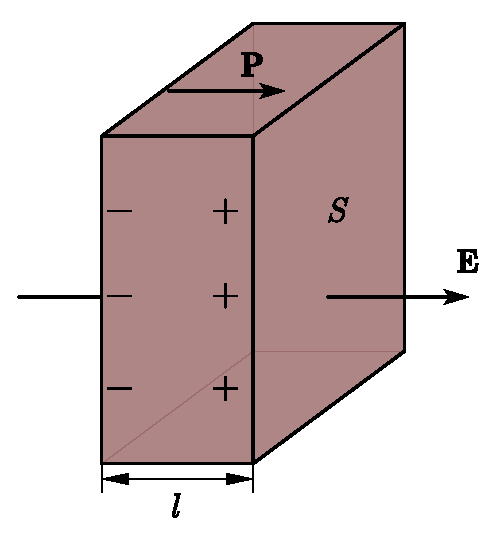
\includegraphics[width=5cm]{./figures/ElePAP_1.pdf}
\caption{极化电荷面密度与电极化强度} \label{ElePAP_fig1}
\end{figure}
设有一厚为$l$、表面积为$S $的电介质薄片\autoref{ElePAP_fig1} 放置在一均匀电场$\mathbf E $中,那么在薄片两表面产生了极化电荷,薄片的电极化强度$\mathbf P $平行于电场强度$\mathbf E$.薄片总的电偶极矩$\sum \mathbf p$是电极化强度的大小与薄片体积的乘积$PSl$,这相当于薄片表面的极化电荷$q' $与薄片两表面正负电荷分开的距离$l $的乘积,即
\begin{equation}
\left|\sum \mathbf p\right|=P S l=q^{\prime} l
\end{equation}
因此,薄片表面的极化电荷面密度就等于电极化强度的大小,即$\sigma^{\prime}=P$.
这个结果假定了薄片表面与$\mathbf P $垂直.在一般情况下,设$\mathbf e_\mathrm{n} $为薄片表面的单位法
向矢量,那么
\begin{equation}
\sigma^{\prime}=\mathbf P \vdot \mathbf e_{\mathrm{n}}=P_{\mathrm{n}}
\end{equation}
即介质极化所产生的极化电荷面密度等于电极化强度沿介质表面外的分量.在薄片侧面,由于$\mathbf P $的方向与侧面法线垂直,所以侧面上的极化电荷面密度为零.